\documentclass[12pt,a4paper]{article}
% Biên dịch: XeLaTeX/Tectonic hoặc pdfLaTeX (vntex).
% TeX Gyre là phông mở đi kèm các bản phân phối TeX thông dụng.
\usepackage{iftex}
\ifPDFTeX
  \usepackage[utf8]{vntex}
  \usepackage{mathptmx}
  \usepackage[scaled=0.92]{helvet}
  \usepackage{courier}
\else
  \usepackage{fontspec}
  \setmainfont{texgyretermes-regular.otf}[
    BoldFont=texgyretermes-bold.otf,ItalicFont=texgyretermes-italic.otf,
    BoldItalicFont=texgyretermes-bolditalic.otf,Ligatures=TeX]
  \setsansfont{texgyreheros-regular.otf}[
    BoldFont=texgyreheros-bold.otf,ItalicFont=texgyreheros-italic.otf,
    BoldItalicFont=texgyreheros-bolditalic.otf,Scale=0.9]
  \setmonofont{texgyrecursor-regular.otf}[
    BoldFont=texgyrecursor-bold.otf,ItalicFont=texgyrecursor-italic.otf,
    BoldItalicFont=texgyrecursor-bolditalic.otf,Scale=0.88]
\fi
\usepackage{amsmath,amssymb}
\ifPDFTeX\else
  \usepackage{unicode-math}
  \setmathfont{texgyretermes-math.otf}
\fi
\usepackage{geometry,graphicx,titlesec}
\usepackage[table]{xcolor}
\usepackage{caption,float,enumitem,tabularx,array,booktabs,indentfirst}
\usepackage{fancyvrb,fancyhdr,microtype}
\geometry{a4paper,left=2.3cm,right=2.3cm,top=2.4cm,bottom=2.3cm,
  headheight=14pt,headsep=16pt,footskip=25pt}
\definecolor{ink}{HTML}{20252B}
\definecolor{darkblue}{HTML}{18384D}
\definecolor{muted}{HTML}{606A73}
\definecolor{lightblue}{HTML}{F2F5F7}
\definecolor{rulegray}{HTML}{CDD3D8}
\color{ink}
\titleformat{\section}{\normalfont\fontsize{14}{17}\selectfont\bfseries}{\thesection}{0.65em}{}
\titleformat{\subsection}{\normalfont\normalsize\bfseries}{\thesubsection}{0.65em}{}
\titlespacing*{\section}{0pt}{14pt}{7pt}
\titlespacing*{\subsection}{0pt}{10pt}{5pt}
\setlength{\fboxsep}{8pt}
\setlength{\fboxrule}{0.4pt}
\newcommand{\infobox}[2][]{\par\smallskip\noindent
  \fcolorbox{rulegray}{lightblue}{\parbox{\dimexpr\linewidth-2\fboxsep-2\fboxrule\relax}{
  \small\textbf{#1}\par\smallskip #2}}\par\smallskip}
\usepackage[unicode,pdfversion=1.7,colorlinks=true,linkcolor=darkblue,urlcolor=darkblue,citecolor=darkblue]{hyperref}
\hypersetup{pdftitle={Thiet ke va kiem chung loi goi he thong tren xv6-riscv},
  pdfauthor={Phan Lê Đăng Khoa; Âu Bảo Trân; Dương Nhựt Duy},
  pdfsubject={Bao cao thuc hanh He dieu hanh -- Lab 02},bookmarksnumbered=true}
\setlength{\parindent}{1.25em}
\setlength{\parskip}{3pt}
\linespread{1.1}
\emergencystretch=1em
\setlist{leftmargin=1.6em,itemsep=2pt,topsep=4pt,parsep=0pt}
\setcounter{tocdepth}{2}
\renewcommand{\contentsname}{Mục lục}
\renewcommand{\figurename}{Hình}
\renewcommand{\tablename}{Bảng}
\renewcommand{\refname}{Tài liệu tham khảo}
\newcolumntype{Y}{>{\raggedright\arraybackslash}X}
\newcolumntype{P}[1]{>{\raggedright\arraybackslash}p{#1}}
\renewcommand{\arraystretch}{1.2}
\setlength{\tabcolsep}{6pt}
\captionsetup{font=small,labelfont=bf,labelsep=period,
  justification=raggedright,singlelinecheck=false,skip=7pt}
\captionsetup[table]{position=top}
\newcommand{\code}[1]{\texttt{#1}}
\DefineVerbatimEnvironment{terminal}{Verbatim}{fontsize=\small,frame=leftline,
  rulecolor=\color{rulegray},framerule=1pt,framesep=9pt,baselinestretch=1.05}
\pagestyle{fancy}
\fancyhf{}
\fancyhead[L]{\sffamily\fontsize{8}{10}\selectfont\color{muted}HỆ ĐIỀU HÀNH\enspace /\enspace LAB 02}
\fancyhead[R]{\sffamily\fontsize{8}{10}\selectfont\color{muted}xv6-riscv}
\fancyfoot[C]{\small\thepage}
\renewcommand{\headrulewidth}{0.3pt}
\renewcommand{\footrulewidth}{0pt}
\fancypagestyle{plain}{\fancyhf{}\fancyfoot[C]{\small\thepage}\renewcommand{\headrulewidth}{0pt}}

\begin{document}
\special{pdf:minorversion 7}
\hypersetup{pageanchor=false}
\begin{titlepage}
\thispagestyle{empty}
\centering
\begin{center}
{\small\bfseries TRƯỜNG ĐẠI HỌC KHOA HỌC TỰ NHIÊN, ĐHQG-HCM}\\[4pt]
{\small KHOA CÔNG NGHỆ THÔNG TIN}
\end{center}
\vspace{0cm}
\begin{center}\includegraphics[width=4cm]{Logo_Truong.png}\end{center}
\vspace*{0.4cm}
{\sffamily\small\bfseries\color{muted}BÁO CÁO THỰC HÀNH HỆ ĐIỀU HÀNH}\\[0.5cm]
{\fontsize{30}{35}\selectfont\bfseries\color{darkblue}Lab 02}\\[0.35cm]
{\fontsize{23}{29}\selectfont\bfseries Thiết kế và kiểm chứng lời gọi\\hệ thống trên xv6-riscv}\\[0.4cm]
{\large\color{muted}System Calls: Trace, Sysinfo, Process Tree}
\par\vspace{0.65cm}
{\color{darkblue}\rule{0.8\textwidth}{0.7pt}}
\par\vspace{0.65cm}
\begin{tabularx}{0.8\textwidth}{@{}p{0.28\textwidth}Y@{}}
\textbf{Lớp} & \textbf{Giảng viên hướng dẫn}\\[3pt]
CQ2024/22 & ThS. Lê Viết Long\\
 & ThS. Phạm Tuấn Sơn\\
\end{tabularx}
\par\vspace{0.65cm}
\textbf{Nhóm thực hiện}\par\smallskip
\begin{tabularx}{0.8\textwidth}{@{}>{\centering\arraybackslash}X>{\centering\arraybackslash}p{3.3cm}@{}}
\toprule
\rowcolor{lightblue}
\textbf{Họ và tên} & \textbf{Mã số sinh viên}\\
\midrule
Phan Lê Đăng Khoa & 24120347\\
Âu Bảo Trân & 24120468\\
Dương Nhựt Duy & 24120293\\
\bottomrule
\end{tabularx}\par
\vfill
{\small\color{muted}Thủ Đức, TP. Hồ Chí Minh -- tháng 11 năm 2026}\par
\end{titlepage}
\pagenumbering{roman}
\hypersetup{pageanchor=true}
\thispagestyle{plain}
\tableofcontents
\clearpage
\pagenumbering{arabic}

\begin{center}
{\large\bfseries Thiết kế và kiểm chứng lời gọi hệ thống trên xv6-riscv}\par
\vspace{4pt}
{\small Phan Lê Đăng Khoa\quad Âu Bảo Trân\quad Dương Nhựt Duy}
\end{center}
\begingroup\small
\noindent\textbf{Tóm tắt.} Báo cáo trình bày ba lời gọi hệ thống bổ sung cho xv6-riscv: theo dõi lời gọi theo bitmask, thu thập bộ nhớ trống và số tiến trình, lấy thông tin để dựng cây tiến trình trong không gian người dùng. Mã nguồn kế thừa Lab 1 và được tích hợp từ ba nhánh có lịch sử riêng. Rà soát phát hiện lỗi kiểm tra giới hạn bộ đệm và byte chưa khởi tạo trong bản ghi process tree; các lỗi được tái hiện trước khi sửa. Thực nghiệm trên QEMU gồm bảy nhóm kiểm thử trace, chín nhóm kiểm thử tích hợp mới, các bộ hồi quy Lab 1 và bộ \code{usertests -q} của xv6. Kết quả kiểm chứng chức năng được ghi theo commit và nhật ký thực thi; báo cáo phân biệt kết quả quan sát với giới hạn về snapshot đồng thời và hiệu năng.
\par\smallskip
\noindent\textbf{Từ khóa:} xv6-riscv; syscall; bitmask; copyout; khóa; cây tiến trình.
\endgroup

\section{Giới thiệu và môi trường}\label{sec:intro}
\subsection{Mục tiêu và phạm vi}
Lab 2 yêu cầu thêm \code{trace}, \code{sysinfo} và \code{ptree}, đồng thời viết các chương trình \code{trace}, \code{sysinfotest} và \code{pstree}. Đề \code{Lab2\_OS\_System\_Call.docx} là căn cứ về chức năng; hướng dẫn MIT năm 2020 được dùng để đối chiếu trace và sysinfo~\cite{assignment,mit-syscall}. Process tree là phần mở rộng trong đề của môn học.

Ba câu hỏi đánh giá gồm: \textbf{RQ1}, trạng thái theo dõi có được giữ đúng qua \code{fork}/\code{exec} và cách ly giữa các tiến trình không; \textbf{RQ2}, dữ liệu kernel có được thu thập dưới khóa phù hợp và chuyển về đúng phạm vi user memory không; \textbf{RQ3}, ba phần có hoạt động cùng nhau và giữ được các chức năng sẵn có không. Báo cáo kiểm chứng tính đúng và xử lý lỗi, không đo hiệu năng hay suy ra điểm môn học.

\subsection{Môi trường và bản mã nguồn}
\begin{table}[H]
\centering\small
\caption{Cấu hình kiểm thử được ghi nhận ngày 04/11/2026.}
\label{tab:environment}
\begin{tabularx}{\textwidth}{@{}P{3.2cm}Y@{}}
\toprule
\rowcolor{lightblue}\textbf{Thành phần} & \textbf{Cấu hình}\\
\midrule
Máy chủ & Ubuntu 24.04.5 LTS, WSL2/Linux 6.6.87.2, x86\_64; AMD Ryzen 5 5600H.\\
Công cụ & RISC-V GCC 13.3.0; QEMU 8.2.2; Python 3.12; GDB đa kiến trúc.\\
Máy giả lập & RISC-V \code{virt}, 128 MiB RAM, 3 CPU ảo; virtio-blk.\\
Baseline nhóm & Lab 1: \code{201dd84}; chuẩn bị chung: \code{fcbb90e}.\\
Bản kiểm chứng & Commit \code{626c6e0}; đầy đủ SHA và lệnh chạy trong \code{docs/lab02/validation/run-context.json}.\\
Giới hạn & \code{NPROC=64}, \code{PGSIZE=4096}, \code{USERSTACK=2}; cấu hình \code{LAB=util} của scaffold được giữ lại.\\
\bottomrule
\end{tabularx}
\end{table}
Giữ \code{LAB=util} bảo toàn cấu hình Lab 1. Chế độ \code{LAB=syscall} trong scaffold MIT 2024 trỏ đến bài \code{attack}, khác đề hiện tại; tên cấu hình không phải số thứ tự lab của môn học. Chỉ các lệnh test được nêu trong báo cáo mới được dùng làm căn cứ kết quả.

\clearpage
\section{Thiết kế và triển khai}\label{sec:design}
\subsection{Đường đi của một lời gọi hệ thống}
Giao diện user được khai báo trong \code{user/user.h}; \code{user/usys.pl} sinh stub đưa số hiệu vào thanh ghi \code{a7} rồi thực hiện \code{ecall}. Sau khi trap vào kernel, dispatcher trong \code{kernel/syscall.c} chọn handler. Handler lấy tham số bằng \code{argint}/\code{argaddr}, xử lý và trả kết quả qua \code{a0}. Cách tổ chức được giữ theo xv6 hiện có~\cite{xv6-book,source}.

\begin{figure}[H]
\centering
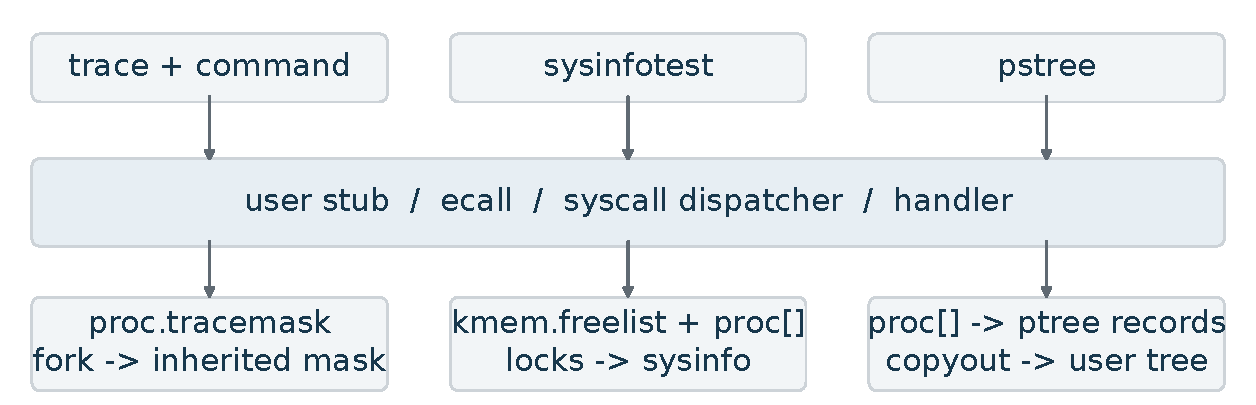
\includegraphics[width=\linewidth]{docs/lab02/figures/architecture.pdf}
\caption{Phân tách xử lý user/kernel của ba syscall; đây là sơ đồ thiết kế, không phải số liệu đo.}
\label{fig:architecture}
\end{figure}

Ba số hiệu được chốt trước khi chia nhánh: \code{SYS\_trace=22} cho trace, \code{SYS\_sysinfo=23} cho sysinfo và \code{SYS\_ptree=24} cho ptree. Tích hợp phải giữ đồng thời bảng handler, bảng tên trace, user stub, prototype và các mục trong \code{UPROGS}; thiếu một mắt xích có thể gây lỗi liên kết hoặc lời gọi không được nhận diện.

\subsection{Trace: trạng thái riêng và kế thừa}
\code{trace(mask)} lưu mask 32 bit trong \code{proc.tracemask}. Với syscall số $s$, điều kiện chọn là bit $s$ của mask được bật. Dispatcher kiểm tra số bit trước phép dịch và log sau khi handler trả về, theo dạng \code{PID: syscall NAME -> RESULT}. Giá trị trả về được in với kiểu có dấu 64 bit để giữ cả kết quả âm.

Mask được khởi tạo khi cấp slot, xóa khi thu hồi và sao chép từ cha trước khi con được chuyển sang runnable. \code{exec} thay không gian địa chỉ nhưng giữ đối tượng process, nên giữ mask. Thay mask ở một process không sửa mask của các process khác. \code{trace(0)} tắt theo dõi; nếu mask mới chứa bit trace thì chính syscall này cũng được log. \code{exit} không trở lại dispatcher nên không có dòng kết quả trả về.

CLI nhận mask thập phân từ 0 đến 2147483647, kiểm tra ký tự và tràn trước phép nhân/cộng. Chương trình chuyển \code{argv+2} trực tiếp cho \code{exec} để giữ các đối số của lệnh đích, trả mã 1 khi usage, mask hoặc exec lỗi. API kernel giữ toàn bộ bit của đối số \code{int}; test riêng bao phủ bit cao và mask $-1$.

\clearpage
\subsection{Sysinfo: thống kê tài nguyên kernel}
\textbf{Giao diện.} \code{sysinfo(struct sysinfo *)} trả 0 khi thành công và $-1$ khi bộ đệm không hợp lệ. Cấu trúc dùng hai trường \code{uint64}: \code{freemem} là số byte bộ nhớ vật lý còn trống; \code{nproc} là số slot có trạng thái khác \code{UNUSED}. Đơn vị byte được giữ thống nhất giữa kernel, chương trình test và báo cáo.

\textbf{Bộ nhớ trống.} Helper trong \code{kernel/kalloc.c} duyệt free list dưới \code{kmem.lock}. Mỗi phần tử tương ứng một trang, nên tổng bằng số trang nhân \code{PGSIZE}. Kết quả không phải tổng RAM giả lập và không tính các trang đã cấp cho kernel, page table, process hoặc pipe là bộ nhớ trống.

\textbf{Số process.} Helper trong \code{kernel/proc.c} duyệt tối đa \code{NPROC} slot. Mỗi slot được kiểm tra dưới \code{p->lock}; chỉ loại \code{UNUSED}. Vì vậy, process đang ngủ, đang chạy hoặc \code{ZOMBIE} chưa được \code{wait} thu hồi đều được tính. Test có đồng bộ pipe để giữ con tồn tại khi đo, và test riêng quan sát zombie trước khi cha gọi wait.

\textbf{Chuyển dữ liệu về user space.} Handler nhận địa chỉ qua \code{argaddr}; đây chỉ là thao tác lấy giá trị tham số, chưa xác nhận con trỏ hợp lệ. Điều kiện phạm vi dùng dạng \code{sizeof(info) <= sz - addr} sau khi kiểm tra \code{addr < sz}, tránh phép cộng có thể tràn. Sau khi điền cấu trúc cục bộ, kernel gọi \code{copyout} và truyền lỗi về nếu trang không tồn tại, là guard page hoặc không có quyền ghi trong user space.

\textbf{Phạm vi đồng thời.} Free list và bảng process được quan sát qua các khóa khác nhau. Không có giao dịch khóa toàn hệ thống bao quanh cả hai phép đếm; vì vậy, hai trường không được hiểu là một ảnh chụp nguyên tử cùng thời điểm. Khi test cần so sánh trước/sau chính xác, tiến trình con được giữ ở trạng thái ổn định bằng pipe và chỉ được giải phóng sau khi đo.

\textbf{Độ phức tạp.} Nếu free list có $F$ trang, chi phí thống kê là $O(F+\mathrm{NPROC})$ và bộ nhớ phụ là $O(1)$. Cách duyệt phù hợp mục đích học thuật và quy mô xv6; báo cáo chưa đo độ trễ hoặc đề xuất dùng syscall này như một bộ giám sát tần suất cao.

\infobox[Kiểm chứng sysinfo]{
Chương trình do thành viên bàn giao kiểm tra dữ liệu cơ bản, cấp/thu hồi bộ nhớ, fork/wait và địa chỉ lỗi, kết thúc bằng \code{sysinfotest: OK}. Test tích hợp bổ sung đơn vị byte, guard page, text chỉ đọc, cấu trúc nằm qua hai trang, giới hạn logical heap và cách đếm zombie.
}

\clearpage
\subsection{Ptree và pstree: tách thu thập khỏi hiển thị}
\textbf{Giao diện dữ liệu.} \code{ptree(buf,max)} trả số bản ghi đã ghi, tối đa \code{max}; trả $-1$ khi đầu vào hoặc copyout lỗi. Mỗi bản ghi chứa PID, PPID, state, kích thước không gian địa chỉ user theo byte và tên 16 byte. Trên ABI RV64 đang dùng, cấu trúc có kích thước 40 byte, gồm cả padding để căn trường 64 bit.

\textbf{Thu thập trong kernel.} Giá trị \code{max<=0} và con trỏ lỗi bị từ chối; max lớn hơn \code{NPROC} được giới hạn về \code{NPROC}. Kernel bỏ các slot UNUSED. Khi đọc quan hệ cha, kernel lấy \code{wait\_lock} trước \code{p->lock}, theo thứ tự đã dùng cho parent pointer trong xv6; thả khóa trước khi copyout. Mỗi bản ghi được zero toàn bộ trước khi điền, bao gồm padding và phần đuôi tên chưa dùng.

\textbf{Giới hạn bộ đệm.} Kiểm tra mapping đơn thuần chưa đủ: sau khi tăng heap một byte, phần còn lại của trang vẫn được map nhưng nằm ngoài \code{sz}. Vì vậy, mỗi đích ghi được kiểm tra với logical size trước khi copyout. Nếu lỗi xuất hiện ở một bản ghi về sau, syscall trả $-1$; những bản ghi trước đó có thể đã được ghi, nên user chỉ sử dụng kết quả khi giá trị trả về không âm.

\textbf{Dựng cây ở user space.} \code{pstree} lấy tối đa 64 bản ghi vào mảng toàn cục, tìm node không có cha trong snapshot rồi in đệ quy với hai khoảng trắng mỗi cấp. Mảng \code{printed} bảo đảm mỗi node chỉ được in một lần; vòng cuối in các node còn lại để xử lý snapshot thiếu parent. Kernel không in cây hoặc giữ bộ đệm trình bày.

Mỗi dòng gồm PID, tên, state dạng số và \code{memsize}. Trường memsize là kích thước không gian địa chỉ user của process, không phải số trang RAM còn trống hoặc RSS. Bản tích hợp bỏ phép ép về \code{int}; hàm in thập phân nhỏ giữ đủ \code{uint64}, vì \code{printf} user trong baseline cũng thu hẹp khi xử lý \code{\%lu}.

\textbf{Chi phí và giới hạn snapshot.} Thu thập có chi phí $O(\mathrm{NPROC})$ và không cấp phát bộ nhớ kernel mới. Dựng cây quét mảng để tìm con nên có chi phí $O(n^2)$, với $n\le64$. Toàn bộ bảng không được đóng băng; khi process exit, exec hoặc reparent trong lúc duyệt, quan hệ giữa các bản ghi có thể thay đổi. Chương trình biểu diễn snapshot thu được, không khẳng định tính nguyên tử toàn hệ thống.

\clearpage
\section{Kiểm thử và đánh giá}\label{sec:testing}
\subsection{Khả năng tái lập và tiêu chí}
Script \code{tools/verify-lab02.py} xuất commit cố định bằng \code{git archive} vào thư mục tạm, chạy clean, build và các bộ test, rồi lưu SHA, cấu hình công cụ, mã thoát và hash nhật ký. Nhờ đó, kết quả không phụ thuộc các object hoặc \code{fs.img} đã có ở checkout làm việc. C được biên dịch với \code{-Wall -Werror}; helper chỉ được cài vào image test, không thêm vào filesystem chuẩn.

\begin{terminal}
python3 tools/verify-lab02.py --commit 626c6e0
\end{terminal}
Các suite có thể chạy riêng bằng các lệnh sau:
\begin{terminal}
make check-trace
make check-lab02
make check-lab01
./grade-lab02-kernel
\end{terminal}
Bộ test làm mới image khi cần, nên dữ liệu thử tay trên image có thể bị thay thế. Kết quả được chấp nhận khi đúng dữ liệu, mã thoát và hoàn tất trong giới hạn thời gian; không coi output mẫu có PID cố định là điều kiện đúng.

\subsection{Ma trận kiểm thử trên bản tích hợp}
\begin{table}[H]
\centering\small
\caption{Các bộ kiểm thử được chạy lại trên cùng commit.}
\label{tab:tests}
\begin{tabularx}{\textwidth}{@{}P{3.0cm}Y P{2.2cm}@{}}
\toprule
\rowcolor{lightblue}\textbf{Bộ kiểm thử} & \textbf{Nội dung và phạm vi} & \textbf{Kết quả}\\
\midrule
Trace, 7 nhóm & Mask đơn/toàn bộ/0, thay mask, fork/exec, sibling, tái sử dụng slot, CLI, forkforkfork. & 7/7; 70/70.\\
Lab 2, 9 nhóm & Sysinfotest của thành viên; heap boundary; sysinfo; ptree; quan hệ và zombie; đồng thời; cây thật; trace hai syscall mới; in 64 bit. & 9/9; 90/90.\\
MIT utility & Các test tương ứng sleep, pingpong, primes kế thừa từ Lab 1. & 5/5.\\
TV1 mở rộng & Đối số, chạy lặp, pipeline, mã thoát và tick của ba tiện ích process. & 5/5; 50/50.\\
Lab 1 tích hợp & cp, diff, tree, du; lỗi tài nguyên, định dạng 64 bit, luồng shell chung. & 7/7; 70/70.\\
Kernel regression & \code{usertests -q} trên kernel tích hợp cả ba syscall. & \code{ALL TESTS PASSED}.\\
\bottomrule
\end{tabularx}
\end{table}
Các điểm trong bảng là thang của script nội bộ, không phải điểm chấm môn học và không cộng thành một điểm đánh giá chung. Nhật ký cuối nằm trong \code{docs/lab02/validation/}; bảng được đối chiếu với kết quả thực thi, không dựa trên việc đã tích ô checklist.

\clearpage
\subsection{Minh chứng chạy thật và phân tích}
Hình~\ref{fig:combined} kiểm chứng bảng tên và handler sau khi ghép nhánh. Mask \code{25165824} chọn bit 23 và 24; cùng một process gọi sysinfo thành công rồi nhận số bản ghi từ ptree. Không có log cho các syscall khác khi mask chỉ chọn hai bit này.

\begin{figure}[H]
\centering
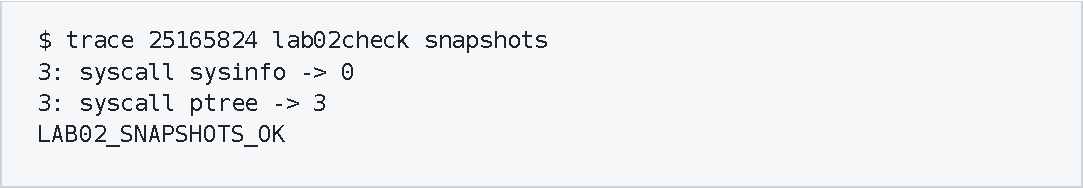
\includegraphics[width=\linewidth]{docs/lab02/figures/combined.pdf}
\caption{Output QEMU được trích từ \code{qemu-combined.txt}; PID có thể thay đổi khi chạy lại.}
\label{fig:combined}
\end{figure}

Hình~\ref{fig:pstree} thể hiện các process init, shell và chính chương trình pstree theo ba mức thụt lề. Đây là cây quan sát tại thời điểm test, không phải cây minh họa được điền thủ công. Các phép kiểm tra PID/PPID nhiều thế hệ dùng pipe giữ process tồn tại; bộ kiểm tra đồng thời thêm fork/exit trong khi hai worker lặp truy vấn snapshot.

\begin{figure}[H]
\centering
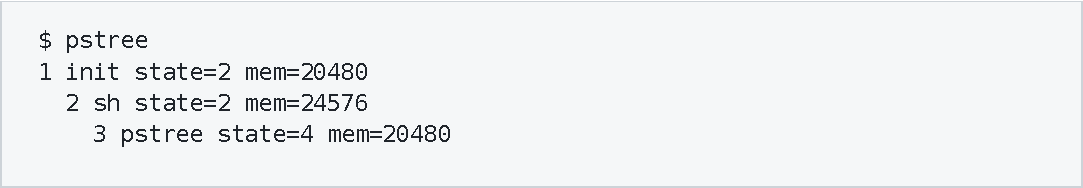
\includegraphics[width=\linewidth]{docs/lab02/figures/pstree.pdf}
\caption{Cây tiến trình thực tế, trích từ \code{qemu-pstree.txt}. State và kích thước phụ thuộc lần chạy.}
\label{fig:pstree}
\end{figure}

\subsection{Lỗi được phát hiện trong rà soát tích hợp}
Hai test trước sửa ghi nhận lỗi có thể tái hiện: ptree nhận buffer ở logical break chưa căn trang và trả các byte đuôi name chưa khởi tạo. Bản sửa thêm kiểm tra \code{sz} cho từng record và zero struct; cùng các test đó đạt sau sửa. Minh chứng trước sửa được giữ ở \code{before-badbuf.txt} và \code{before-ptree.txt}; các phép kiểm tra cuối bổ sung cả padding, guard page và text không có quyền ghi.

Một lỗi về độ rộng dữ liệu được xử lý bằng cách giữ memsize 64 bit đến lúc in. Test formatter dùng $2^{32}$ và $2^{64}-1$ để phát hiện thu hẹp kiểu; các giá trị này là dữ liệu tổng hợp cho hàm trình bày, không phải bộ nhớ process thật trên máy giả lập 128 MiB.

\clearpage
\section{Khó khăn và giới hạn}\label{sec:limits}
\textbf{Tích hợp trên cùng file.} Ba nhánh cùng thêm dispatcher, stub và prototype. Xung đột được giải quyết bằng cách giữ đủ ba syscall cùng ID đã thống nhất, không chọn toàn bộ file của một nhánh để thay phần còn lại. Nhánh ptree còn có thay đổi CRLF rộng và xóa file nguồn báo cáo Lab 1; merge chuẩn hóa LF, giữ lại báo cáo cũ và thêm quy ước line ending. Các commit gốc của thành viên vẫn là tổ tiên của bản tích hợp.

\textbf{Con trỏ và byte padding.} Dữ liệu có mapping chưa chắc nằm trong logical heap; một cấu trúc có tất cả trường hợp lệ vẫn có thể chứa padding chưa khởi tạo. Hai vấn đề này cần kiểm thử riêng, không chỉ kiểm tra output cây hoặc dòng \code{sysinfotest: OK}. Dùng \code{copyout} là điều kiện cần để kiểm tra page và quyền truy cập; kiểm tra phạm vi và khởi tạo buffer vẫn phải làm ở handler/helper.

\textbf{Đồng thời và hiệu năng.} Việc lấy từng khóa giúp bảo vệ cấu trúc đang đọc, nhưng không tạo snapshot nguyên tử giữa tất cả slot hoặc giữa bộ nhớ và process. Số PID, state, freemem và thời gian hoàn tất có thể thay đổi. Trace phát sinh console I/O và có thể làm đổi lịch thực thi. Các test đồng thời đã đạt chỉ bao phủ các workload đã chạy, không chứng minh mọi xen kẽ hoặc độ trễ tối đa.

\section{Phân công và đóng góp}\label{sec:contribution}
\begin{table}[H]
\centering\small
\caption{Phần bàn giao theo phân công và lịch sử Git.}
\label{tab:contribution}
\begin{tabularx}{\textwidth}{@{}P{3.25cm}Y@{}}
\toprule
\rowcolor{lightblue}\textbf{Thành viên} & \textbf{Phần triển khai được ghi nhận}\\
\midrule
Phan Lê Đăng Khoa & Trace, chương trình trace và self-test; nhánh \code{lab2-trace}, head \code{0d06ca9}. Theo phân công phụ trách điều phối và tích hợp.\\
Âu Bảo Trân & Sysinfo, helper thống kê bộ nhớ/process, sysinfotest; nhánh \code{lab2-sysinfo}, commit \code{05da92d}.\\
Dương Nhựt Duy & Ptree, header dữ liệu và pstree; nhánh \code{lab2-ptree}, head \code{c0a4bb7}.\\
\bottomrule
\end{tabularx}
\end{table}
Các sửa lỗi, test bổ sung và chuẩn hóa khi tích hợp được ghi trong commit \code{626c6e0} và \code{docs/lab02/REVIEW.md}. Bảng ghi nhận phạm vi bàn giao từ Git, không quy đổi số dòng hay số commit thành phần trăm đóng góp. Rà soát kỹ thuật tích hợp trong hồ sơ không thay cho biên bản review chéo mang tên từng thành viên.

\clearpage
\section{Kết luận}
Lab 2 đã bổ sung đủ ba syscall trên cùng kernel xv6-riscv. Trace minh họa trạng thái riêng của process và tính kế thừa; sysinfo nối thống kê kernel với bộ đệm user; ptree phân tách thu thập thông tin khỏi dựng cây. Bản tích hợp giữ lịch sử ba nhánh và vượt qua các bộ test chức năng cùng hồi quy được nêu trong Bảng~\ref{tab:tests}.

Kết quả rà soát cho thấy kiểm tra mapping, kiểm tra logical size và khởi tạo dữ liệu trước copyout là ba trách nhiệm khác nhau. Đầu ra đúng trong trường hợp thông thường chưa đủ phát hiện lỗi padding hoặc bộ đệm nằm ngoài heap nhưng còn trong trang. Các giới hạn còn lại gồm snapshot không nguyên tử, khả năng đã ghi một phần khi copyout lỗi và tác động I/O của trace; chưa có kết quả đo hiệu năng hoặc chứng minh đầy đủ tính đúng đồng thời.

\phantomsection
\addcontentsline{toc}{section}{Tài liệu tham khảo}
\begingroup\small\raggedright
\begin{thebibliography}{9}
\setlength{\itemsep}{7pt}
\bibitem{assignment} Đề bài môn Hệ điều hành, \emph{Project 2 -- System call}, \code{Lab2\_OS\_System\_Call.docx}. Yêu cầu trace, sysinfo, process tree và quy định bài nộp.
\bibitem{mit-syscall} MIT, \emph{Lab: System calls}, 6.S081, 2020. Đối chiếu hướng dẫn trace/sysinfo ngày 04/11/2026.\\
\url{https://pdos.csail.mit.edu/6.828/2020/labs/syscall.html}
\bibitem{xv6-book} R. Cox, F. Kaashoek, R. Morris, \emph{xv6: a simple, Unix-like teaching operating system}, bản RISC-V, 2024. Chương 2--4 và 6 dùng để đối chiếu tổ chức kernel, syscall, đối số và thứ tự khóa. Truy cập ngày 04/11/2026.\\
\url{https://pdos.csail.mit.edu/6.1810/2024/xv6/book-riscv-rev4.pdf}
\bibitem{source} Nhóm thực hiện, \emph{Mã nguồn và hồ sơ Lab 2}, commit kiểm chứng \code{626c6e0}; các nhánh thành viên, \code{docs/lab02/REVIEW.md} và chương trình kiểm thử trong \code{tests/}.\\
\url{https://github.com/EndlessMelody/os-lab2}
\bibitem{evidence} Nhóm thực hiện, \emph{Minh chứng kiểm thử và báo cáo ngày 04/11/2026}, \code{docs/lab02/validation/} và \code{docs/lab02/figures/}. Lệnh, mã thoát, SHA commit và hash nhật ký lưu trong \code{run-context.json}; figure có hồ sơ nguồn và dòng trích trong \code{manifest.json}.
\end{thebibliography}
\endgroup
\end{document}
